\documentclass[]{article}

%opening
\title{Linear Regression}
\author{onerhao}

\usepackage{amssymb,amsmath,bm,amsthm}
\usepackage{textcomp}
\usepackage{longtable}
\usepackage{algorithm2e}
\usepackage{tocbibind}
\usepackage[toc]{multitoc}
\usepackage{mathptmx}        % selects Times Roman as basic font
\usepackage{helvet}          % selects Helvetica as sans-serif font
\usepackage{courier}         % selects Courier as typewriter font
%\usepackage{type1cm}        % activate if the above 3 fonts are 
% not available on your system

\usepackage{makeidx}         % allows index generation
\usepackage{graphicx}        % standard LaTeX graphics tool
% when including figure files
\usepackage[justification=centering]{caption}
\usepackage{subfig}
\usepackage{multicol}        % used for the two-column index
\usepackage{multirow}
\usepackage[bottom]{footmisc}% places footnotes at page bottom
\usepackage[bookmarksnumbered=true,
bookmarksopen=true,
colorlinks=true,
linkcolor=blue,
anchorcolor=blue,
citecolor=blue
]{hyperref}

\begin{document}

\maketitle

\begin{abstract}

\end{abstract}


\section{Introduction}
Linear regression is the “work horse” of statistics and (supervised) machine learning. When augmented with kernels or other forms of basis function expansion, it can model also nonlinear relationships. And when the Gaussian output is replaced with a Bernoulli or multinoulli distribution, it can be used for classification, as we will see below. So it pays to study this model in detail.


\section{Representation}

\begin{equation}
p(y|\vec{x},\vec{\theta})=\mathcal{N}(y|\vec{w}^T\vec{x}, \sigma^2)
\end{equation}
where $\vec{w}$ and $\vec{x}$ are extended vectors, $\vec{x}=(1,x)$, $\vec{w}=(b,w)$.

Linear regression can be made to model non-linear relationships by replacing $\vec{x}$ with some non-linear function of the inputs, $\phi(\vec{x})$ \begin{equation}
p(y|\vec{x},\vec{\theta})=\mathcal{N}(y|\vec{w}^T\phi(\vec{x}), \sigma^2)
\end{equation}

This is known as \textbf{basis function expansion}. (Note that the model is still linear in the parameters $\vec{w}$, so it is still called linear regression; the importance of this will become clear below.) A simple example are polynomial basis functions, where the model has the form
\begin{equation}
\phi(x)=(1, x, \cdots, x^d)
\end{equation}



\section{Maximum likelihood estimations(least squares)}
A common way to estimate the parameters of a statistical model is to compute the MLE,which is defined as
\begin{equation}
\vec{\hat{\theta}}=\arg\max_\theta{logp(D|\vec{\theta})}
\end{equation}
Assume the training examples are \textbf{independently and identically distributed(IID)},we can write the \textbf{log-likelihood} function as follows:
\begin{equation}
\ell(\vec{\theta}) \triangleq \log p(\mathcal{D}|\vec{\theta})
\end{equation}
Instead of maximizing the log-likelihood, we can equivalently minimize the \textbf{negative log likelihood} or \textbf{NLL}:
\begin{equation}
\text{NLL}(\vec{\theta}) \triangleq -\ell(\vec{\theta})=-\log p(\mathcal{D}|\vec{\theta})
\end{equation}

The NLL formulation is sometimes more convenient, since many optimization software packages are designed to find the minima of functions, rather than maxima.

Now let us apply the method of MLE to the linear regression setting. Inserting the definition of the Gaussian into the above, we find that the log likelihood is given by
\begin{align}
\ell(\vec{\theta})& =\sum\limits_{i=1}^N \log\left[\dfrac{1}{\sqrt{2\pi}\sigma}\exp\left(-\dfrac{1}{2\sigma^2}(y_i-\vec{w}^T\vec{x}_i)^2\right)\right] \\
& =-\dfrac{1}{2\sigma^2}\text{RSS}(\vec{w})-\dfrac{\vec{w}}{2}\log(2\pi\sigma^2)
\end{align}

RSS stands for \textbf{residual sum of squares} and is defined by
\begin{equation}
\text{RSS}(\vec{w}) \triangleq \sum\limits_{i=1}^N (y_i-\vec{w}^T\vec{x}_i)^2
\end{equation}

We see that the MLE for $\vec{w}$ is the one that minimizes the RSS, so this method is known as \textbf{least squares}.

Let's drop constants wrt $\vec{w}$ and NLL can be written as
\begin{equation}
\text{NLL}(\vec{w}) = \dfrac{1}{2}\sum\limits_{i=1}^N (y_i-\vec{w}^T\vec{x}_i)^2
\end{equation}

There two ways to minimize NLL$(\vec{w})$.


\subsection{Derivations of the MLE}
Define $\vec{y}=(y_1,y_2,\cdots,y_N)$, $\vec{X}=\left(\begin{array}{c}\vec{x}_1^T \\ \vec{x}_2^T \\ \vdots \\ \vec{x}_N^T\end{array}\right)$, then we can rewritten the objective in a form that is more amendable to differentiation:
\begin{align}
\text{NLL}(\vec{w}) &= \dfrac{1}{2}(\vec{y}-\vec{X}\vec{w})^T(\vec{y}-\vec{X}\vec{w})\\
&= \dfrac{1}{2} [\vec{w^T} (\vec{X}^T\vec{X})\vec{w} - \vec{y}^T\vec{x}\vec{w}- \vec{w}^T\vec{x}^T\vec{y}  +\vec{y}^T\vec{y}]			\\
\Rightarrow
\dfrac{\partial}{\partial \vec{w}}\text{NLL} &= \dfrac{1}{2} \vec{w^T} (\vec{X}^T\vec{X})\vec{w} -\vec{w}^T(\vec{x}^T\vec{y}) 
\end{align}

where
$\begin{cases}
\vec{X} = \begin{bmatrix}
&\vec{x_1^T} \\
&\vec{x_2^T} \\
& ... \\
&\vec{x_n^T}
\end{bmatrix}\\	
\vec{X^T}\vec{X} =
\begin{bmatrix}
\vec{x_1} & \vec{x_2} & ...&\vec{x_n}
\end{bmatrix} 
\cdot
\begin{bmatrix}
&\vec{x_1^T} \\
&\vec{x_2^T} \\
& ... \\
&\vec{x_n^T}
\end{bmatrix}  = \sum\limits_{i=1}^{N}\vec{x_i}\vec{x_i^T} = \sum\limits_{i=1}^{N} \\
\end{cases}$
is the \textbf{sum of squares } matrix.

When $\mathcal{D}$ is small(for example, $N < 1000$), we can use the following equation to compute $\vec{w}$ directly
\begin{equation}
\hat{\vec{w}}_{\mathrm{OLS}}=(\vec{X}^T\vec{X})^{-1}\vec{X}^T\vec{y}
\end{equation}

The corresponding solution $\hat{\vec{w}}_{\mathrm{OLS}}$ to this linear system of equations is called the \textbf{ordinary least squares} or \textbf{OLS} solution.

\begin{proof}
	We now state without proof some facts of matrix derivatives (we won’t need all of these at this section).
	\begin{eqnarray}
	trA &\triangleq& \sum\limits_{i=1}^n A_{ii} \nonumber \\
	\frac{\partial}{\partial A}AB &=& B^T \\
	\frac{\partial}{\partial A^T}f(A) &=& \left[\frac{\partial}{\partial A}f(A)\right]^T \label{eqn:matrix-1} \\
	\frac{\partial}{\partial A}ABA^TC &=& CAB+C^TAB^T \label{eqn:matrix-2} \\
	\frac{\partial}{\partial A}|A| &=& |A|(A^{-1})^T
	\end{eqnarray}
	
	Then,
	\begin{eqnarray*}
		\text{NLL}(\vec{w}) &=& \frac{1}{2N}(\vec{X}\vec{w}-\vec{y})^T(\vec{X}\vec{w}-\vec{y}) \\
		\frac{\partial \text{NLL}}{\partial\vec{w}} &=& \frac{1}{2} \frac{\partial}{\partial\vec{w}} (\vec{w}^T\vec{X}^T\vec{X}\vec{w}-\vec{w}^T\vec{X}^T\vec{y}-\vec{y}^T\vec{X}\vec{w}+\vec{y}^T\vec{y}) \\
		&=& \frac{1}{2} \frac{\partial}{\partial\vec{w}} (\vec{w}^T\vec{X}^T\vec{X}\vec{w}-\vec{w}^T\vec{X}^T\vec{y}-\vec{y}^T\vec{X}\vec{w}) \\
		&=& \frac{1}{2} \frac{\partial}{\partial\vec{w}} tr(\vec{w}^T\vec{X}^T\vec{X}\vec{w}-\vec{w}^T\vec{X}^T\vec{y}-\vec{y}^T\vec{X}\vec{w}) \\
		&=& \frac{1}{2} \frac{\partial}{\partial\vec{w}} (tr\vec{w}^T\vec{X}^T\vec{X}\vec{w}-2tr\vec{y}^T\vec{X}\vec{w})
	\end{eqnarray*}
	
	Combining Equations \ref{eqn:matrix-1} and \ref{eqn:matrix-2}, we find that 
	\begin{equation*}
	\frac{\partial}{\partial A^T}ABA^TC = B^TA^TC^T+BA^TC
	\end{equation*}
	
	Let $A^T=\vec{w}, B=B^T=\vec{X}^T\vec{X}$, and $C=I$, Hence,
	\begin{eqnarray}
	\frac{\partial \text{NLL}}{\partial\vec{w}} &=& \frac{1}{2} (\vec{X}^T\vec{X}\vec{w}+\vec{X}^T\vec{X}\vec{w} -2\vec{X}^T\vec{y}) \nonumber \\
	&=& \frac{1}{2} (\vec{X}^T\vec{X}\vec{w} - \vec{X}^T\vec{y}) \nonumber \\
	\frac{\partial \text{NLL}}{\partial\vec{w}} &=& 0 \Rightarrow \vec{X}^T\vec{X}\vec{w} - \vec{X}^T\vec{y} =0 \nonumber \\
	\vec{X}^T\vec{X}\vec{w} &=& \vec{X}^T\vec{y} \label{eqn:normal-equation} \\
	\hat{\vec{w}}_{\mathrm{OLS}} &=& (\vec{X}^T\vec{X})^{-1}\vec{X}^T\vec{y} \nonumber
	\end{eqnarray}
\end{proof}
Equation \ref{eqn:normal-equation} is known as the \textbf{normal equation}.
\begin{proof}
	Consider $\mathbf{vector-vector}$ differentiation,if $\mathbf{A}$ is not a function of $\vec{x}$ then
	\begin{equation}
	\dfrac{\partial\vec{X}^TA\vec{X}}{\partial\vec{X}} = \vec{X}^T(\mathbf{A}+\mathbf{A}^T) = (\mathbf{A}+\mathbf{A}^T)\vec{X}
	\end{equation}
\end{proof}
Then,we can derivate $\dfrac{\partial NLL}{\partial \vec{w}}$
\begin{eqnarray}
g(\vec{w}) &= \dfrac{\partial NLL}{\partial\vec{w}} \\
&=\vec{X}^T\vec{X}\vec{w} - \vec{X}^T\vec{y}			
\end{eqnarray}
Setting the derivative to zero,we get
\begin{equation}
\vec{w} = (\vec{X}^T\vec{X})^{-1}\vec{x}^T\vec{y}
\end{equation}

\subsubsection{Geometric interpretation}

See Figure \ref{fig:graphical-interpretation-of-OLS}.
\begin{figure}[hbtp]
	\centering
	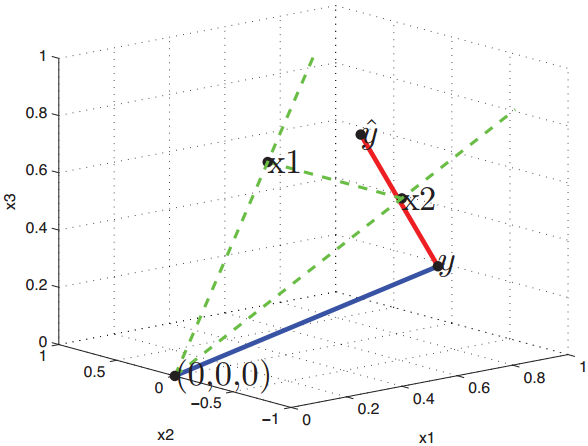
\includegraphics[scale=.50]{graphical-interpretation-of-OLS.png}
	\caption{Graphical interpretation of least squares for $N=3$ examples and $D=2$ features. $\tilde{\vec{x}}_1$ and $\tilde{\vec{x}}_2$˜ are vectors in $\mathbb{R}^3$; together they define a 2D plane. $\vec{y}$ is also a vector in $\mathbb{R}^3$ but does not lie on this 2D plane. The orthogonal projection of $\vec{y}$ onto this plane is denoted $\hat{\vec{y}}$. The red line from $\vec{y}$ to $\hat{\vec{y}}$ is the residual, whose norm we want to minimize. For visual clarity, all vectors have been converted to unit norm.}
	\label{fig:graphical-interpretation-of-OLS} 
\end{figure}

To minimize the norm of the residual, $\vec{y}-\hat{\vec{y}}$, we want the residual vector to be orthogonal to every column of $\vec{X}$,so˜ $\tilde{\vec{x}}_j(\vec{y}-\hat{\vec{y}})=0$ for $j=1:D$. Hence
\begin{equation}\begin{split}
\tilde{\vec{x}}_j(\vec{y}-\hat{\vec{y}})=0 & \Rightarrow \vec{X}^T(\vec{y}-\vec{X}\vec{w})=0 \\
& \Rightarrow \vec{w}=(\vec{X}^T\vec{X})^{-1}\vec{X}^T\vec{y}
\end{split}\end{equation}


\subsection{SGD}
When $\mathcal{D}$ is large, use stochastic gradient descent(SGD).

\begin{align}
\because \dfrac{\partial}{\partial w_i}\text{NLL}(\vec{w})=& \sum\limits_{i=1}^N (\vec{w}^T\vec{x}_i-y_i)x_{ij} \\
\therefore w_j=& w_j - \alpha\dfrac{\partial}{\partial w_j}\text{NLL}(\vec{w}) \nonumber \\
=& w_j - \sum\limits_{i=1}^N \alpha(\vec{w}^T\vec{x}_i-y_i)x_{ij} \\
\therefore \vec{w}=& \vec{w}-\alpha(\vec{w}^T\vec{x}_i-y_i)\vec{x}
\end{align}


\end{document}
